% =========================================================================== %

\begin{frame}[t,plain]
\titlepage
\end{frame}

% =========================================================================== %

\begin{frame}{Recap}
%
\begin{columns}[T]
\column{.5\linewidth}
\begin{itemize}
\item Generator Objects
	\begin{itemize}
	\item List comprehension syntax in (parentheses)
	\item Object compatible with \inPy{for} and \inPy{next}
	\item Not subscriptable
	\item Will get depleted
	\item Stores code, not results
	\end{itemize}
\item \inPy{yield}
	\begin{itemize}
	\item Similar to \inPy{return}
	\item Makes generator object from function
	\end{itemize}
\end{itemize}
%
\column{.5\linewidth}
\begin{itemize}
\item Iterable classes
	\begin{itemize}
	\item Implicit calls to \inPy{iter} and \inPy{next} by \inPy{for}
	\item Dunder \inPy{__iter__}: Returns helper object with \inPy{__next__}
	\item Dunder \inPy{__next__}: Computes next in line and updates helper object
	\item Helper object usually has \inPy{__iter__} which returns \inPy{self}
	\end{itemize}
\end{itemize}

\end{columns}
%
\begin{center}
	\emph{Any Questions?}
\end{center}
%
\end{frame}

% =========================================================================== %

\begin{frame}
%
\begin{center}
	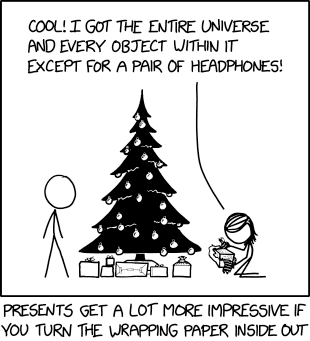
\includegraphics[width=.35\linewidth]{./gfx/xkcd-wrappingPaper}
	
	\emph{Wow, rude of you to regift literally every gift that you or anyone else has ever received.}

	\vspace{6pt}
	Source: \url{https://xkcd.com/2403/}
\end{center}
%
\end{frame}

% =========================================================================== %

\begin{frame}{Scenarios}
%
\begin{itemize}
\item Extensions
	\begin{itemize}
	\item You've got a function
	\item You want to add some feature to it
	\item You want to add the same feature to other functions as well
	\end{itemize}
\item Closed source
	\begin{itemize}
	\item You want to do the above to some library function
	\end{itemize}
\item Classes
	\begin{itemize}
	\item You want to do the above to some class(es)
	\end{itemize}
\item Parametrization
	\begin{itemize}
	\item You want to change the number of arguments a function takes
	\end{itemize}
\end{itemize}
%
\end{frame}

% =========================================================================== %

\begin{frame}[fragile]
%
\begin{columns}[T]
\column{.5\linewidth}
\begin{Large}
	{Recap: Functions as Objects}
	\vspace{12pt}
\end{Large}
\begin{itemize}
\item Functions are stored \emph{somehwere} in memory
\item So they can be handled like any other data object
\item Can be stored in a variable
\item Can be passed to other functions
\item Can be returned as results
\end{itemize}
%
\column{.5\linewidth}
\begin{codebox}[Example: Passing Functions]
\begin{minted}[fontsize=\scriptsize, linenos]{python3}
def foobar () :
    print("This is foobar")

def doSomething (func) :
    print("This is doSomething")
    func()
    print("doSomething again")

doSomething(foobar)
\end{minted}
\end{codebox}
%
\begin{cmdbox}[Output: Passing Functions]
\begin{minted}[fontsize=\scriptsize]{text}
This is doSomething
This is foobar
doSomething again
\end{minted}
\end{cmdbox}
\end{columns}
%
\end{frame}

% =========================================================================== %

\begin{frame}[fragile]
%
\begin{tcbraster}[raster columns=2,
                  raster equal height,
                  nobeforeafter,
                  raster column skip=0.5cm]
\begin{codebox}[Scheme: Returning Functions]
\begin{minted}[fontsize=\scriptsize, linenos]{python3}
def outer (param) :
    def inner():
        return param
    return inner

x = outer(1)
y = outer(2)

print( "x:", x, "returns", x() )
print( "y:", y, "returns", y() )
\end{minted}
\end{codebox}
%
\begin{cmdbox}[Output: Returning Functions]
\begin{minted}[fontsize=\scriptsize]{text}
x: <function outer.<locals>.inner at 
    0x7f800a0c6700> returns 1
y: <function outer.<locals>.inner at
    0x7f800a0ea700> returns 2
\end{minted}
\end{cmdbox}
\end{tcbraster}
%
\begin{itemize}
\item \texttt{outer} computes and returns \texttt{inner}
\item Makes a new copy every time (cf. adresses!)
\item \texttt{outer} has its internal set of variables \texttt{<locals>}
\end{itemize}
%
\end{frame}

% =========================================================================== %

\begin{frame}[fragile]
%
\begin{codebox}[Example: Numerical Derivative, width=.60\linewidth, nobeforeafter, equal height group = grpNumDerivative]
\begin{minted}[linenos, fontsize=\scriptsize]{python}
import numpy as np
import matplotlib.pyplot as plt

def derivative (f, epsilon = 1e-7) :
    def result(x) :
        return (f(x + epsilon) - f(x)) / epsilon
    return result

dtan = derivative(np.tan)

X = np.linspace(-6.28, 6.28, 251)
Y = dtan(X)

plt.plot(X, Y)
plt.show()
\end{minted}
\end{codebox}
%
\begin{tcolorbox}[title=Output: Num. Derivative, width=.39\linewidth, nobeforeafter, equal height group = grpNumDerivative]
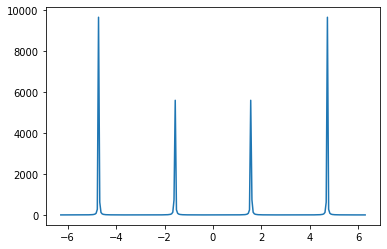
\includegraphics[width=\linewidth]{./gfx/numDerivativeTan}
\end{tcolorbox}
%
Decorators: Definition for mathematicians
\begin{itemize}
\item $\mathcal{F}$: space of functions
\item Decorator: $D : \mathcal{F} \to \mathcal{F}$
\end{itemize}
%
\end{frame}

% =========================================================================== %

\begin{frame}[fragile]
%
\begin{columns}[T]
\column{.5\linewidth}
\begin{Large}
	{Overwriting Symbols}
	\vspace{6pt}
\end{Large}
%
\begin{itemize}
\item Assume: For debug: print arguments and result on screen
\item Do so for multiple functions
\item[\Thus] Wrap debug code around useful code
\item Later: want to remove debug output
\item[\Thus] Temporarily overwrite \emph{symbols}
\item Original code remains in memory, but \emph{anonymously}
\item Line 2: create new function that is returned in line 16
\item Symbol \texttt{stuff} refers to \emph{new} function
\item New function still refers to adress of \emph{old} function
\end{itemize}
%
\column{.5\linewidth}
\begin{codebox}[Example: Debug Wrapper]
\begin{minted}[fontsize=\scriptsize, linenos]{python3}
def debug (func) :
  def wrapper (*args, **kwargs) :
    print(f"Call to {func.__name__}")
    
    print( "   with arguments:")
    for arg in args : print(" *", arg)
    
    print( "   keyword arguments:")
    for key, val in kwargs.items() :
      print(" *", key, "=", val)
    
    result = func(*args, **kwargs)
    print("returns", result)
    return result
        
  return wrapper

def stuff () :
    print("This is stuff")

stuff = debug(stuff)
\end{minted}
\end{codebox}
\end{columns}
%
\end{frame}

% =========================================================================== %

\begin{frame}[fragile]{Short Syntax for Decorators}
%
\begin{columns}[T]
\column{.5\linewidth}
\begin{itemize}
\item New syntax element: \inPy{@decorator}
\item Placed before definition of undecorated function
\item automatically causes \inPy{function = decorator(function)}
\end{itemize}
%
\column{.5\linewidth}
\begin{codebox}[Schema: Decorators]
\begin{minted}[fontsize=\scriptsize]{python3}
def decorator (func) :
    def wrapper (params) :
        ... func(params) ...
    return wrapper

@decorator
def funcToDecorate(params) :
    undecorated code
\end{minted}
\end{codebox}
\end{columns}
%
\end{frame}

% =========================================================================== %

\begin{frame}[fragile]
%
\begin{codebox}[Example: Call Counter, width=.60\linewidth, nobeforeafter, equal height group = grpCallCounter]
\begin{minted}[linenos, fontsize=\scriptsize]{python3}
def callCounter (func) :
    counter = 0
    def wrapper (*args, **kwargs) :
        nonlocal counter
        counter += 1
        return counter, func(*args, **kwargs)
    return wrapper

@callCounter
def foo () :
    print("foo")

@callCounter
def bar () :
    print("bar")

print( foo() )
print( foo() )
print( bar() )
print( foo() )
\end{minted}
\end{codebox}
%
\begin{cmdbox}[Output: Call Counter, width=.39\linewidth, nobeforeafter, equal height group = grpCallCounter]
\begin{minted}[fontsize=\scriptsize]{text}
foo
(1, None)
foo
(2, None)
bar
(1, None)
foo
(3, None)
\end{minted}
\end{cmdbox}
%
\end{frame}

% =========================================================================== %

\begin{frame}{How Does This Work?}
%
\begin{itemize}
\item Each function call: \emph{allocates} new memory for all variables
\item Binding: assign code symbols to these memory locations
\item On exit: unbind and deallocate all \emph{unreferenced} variables
	\begin{itemize}
	\item Unreferenced if no active symbol is bound the memory location
	\item Recursively kept \enquote{alive}!
	\end{itemize}
\item \inPy{@callCounter}, \inPy{def foo () :}
	\begin{itemize}
	\item New allocation and binding of \texttt{counter}
	\item \inPy{nonlocal counter} binds symbol in \texttt{wrapper} to the variable of \texttt{callCounter}
	\item \texttt{foo} stays \enquote{alive}, and so do \emph{the memory location} of \texttt{callCounter}
	\end{itemize}
\item \inPy{@callCounter}, \inPy{def bar () :}
	\begin{itemize}
	\item Again: new allocation
	\item Get a brand new \texttt{counter} \emph{without affecting} the old one!
	\end{itemize}
\end{itemize}
%
\end{frame}

% =========================================================================== %

\begin{frame}[fragile]{Parametrized Decorators}
%
\begin{itemize}
\item So far: Decorator
	\begin{itemize}
	\item Function that takes a function and computes a function
	\item Takes exactly one argument
	\item Returns exactly one function
	\item @-Syntax works only in this case
	\end{itemize}
\item What if Decorator needs additional argument(s)?
	\begin{itemize}
	\item Example: n-fold execution
	\item We then need to \emph{compute a decorator}!
	\item Three levels of nested functions
	\item First level: computes decorator
	\item Second level: computes decorated function
	\item Third level: computes decorated result
	\end{itemize}
\end{itemize}
%
\end{frame}

% =========================================================================== %

\begin{frame}[fragile]{Example: Taylor Series}
%
\begin{itemize}
\item Most functions can be written in terms of polynomials
\item[\Thus] Taylor series
\item Infinite Sum:
	\begin{align*}
	f(x) = \sum_{n=0}^{\infty} \frac{f^{(n)}(a)}{n!} (x - a)^n
	\end{align*}
\item Computer can only do a \emph{finite} sum
\item[\Thus] Parameter $N$ (upper limit for summation)
\item Provide $f^{(n)}(a)$ for a given $a$ (usually $a = 0$)
\item (Or, entire summand -- easier to grasp in the following example)
\end{itemize}
%
\end{frame}

% =========================================================================== %

\begin{frame}[fragile]
%
\begin{tcbraster}[raster columns=2,
                  raster equal height,
                  nobeforeafter,
                  raster column skip=0.2cm]
\begin{codebox}[Example: Sine Series]
\begin{minted}[linenos, fontsize=\scriptsize]{python3}
import numpy as np
import matplotlib.pyplot as plt

plt.rcParams["figure.figsize"] = (10,7)

N = 10
approximations = []
X = np.linspace(0, 2*np.pi, 314)

def makeSeries (N) :
  def decorator(expr) :
    def wrapper(*args, **kwargs) :
      result = 0
      for n in range(N) :
        result += expr(n,*args,**kwargs)
        return result
    return wrapper
  return decorator
\end{minted}
\end{codebox}
%
\begin{codebox}[... continued]
\begin{minted}[fontsize=\scriptsize, linenos, firstnumber=last]{python3}
for n in range(1, N) :
  @makeSeries(n)
  def sine(n, x) :
    return ((-1)**n / \
      np.math.factorial(2*n + 1)) * \
      x**(2*n + 1)
    
  approximations.append(sine)

for n, sin in enumerate(approximations) :
    plt.plot(X, sin(X),
             label=f"degree {n+1}",
             color=f"#0088{n}{n}ff")

plt.ylim(-1.5, +1.5)
plt.plot(X, np.sin(X),
         label="numpy sin",
         color='r')
plt.legend(loc="lower left")
plt.show()
\end{minted}
\end{codebox}
\end{tcbraster}
%
\end{frame}

% =========================================================================== %

\begin{frame}
%
\begin{tcolorbox}[title=Output: Sine Series]
\begin{center}
	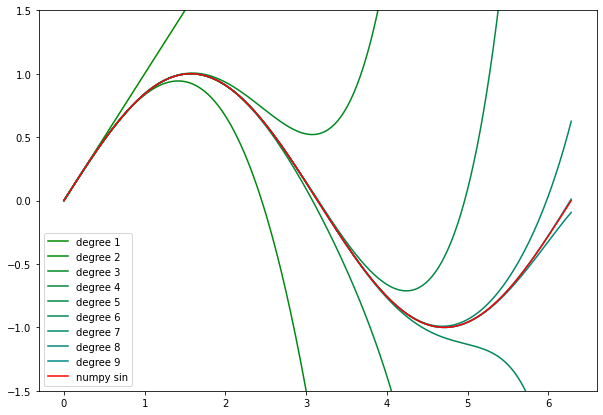
\includegraphics[width=.7\linewidth]{./gfx/sin-taylor}
\end{center}
\end{tcolorbox}
%
\end{frame}

% =========================================================================== %

\begin{frame}[fragile]
%
\begin{columns}[T]
\column{.5\linewidth}
\begin{Large}
	{Stacking Decorators}
	\vspace{12pt}
\end{Large}
\begin{itemize}
\item Simply by multiple \texttt{@}-lines
\item First decoarator wraps around second wraps around ... func
\item Arbitrary count of decorators
\item Order does matter
\item Imagine \emph{decorated} decorator
\end{itemize}
%
\vspace{15pt}
\begin{codebox}[Example: Order of Decorators]
\begin{minted}[fontsize=\scriptsize, linenos]{python3}
indentLevel = 0

def printIndented(*args, **kwargs) :
  print("   " * indentLevel,
        *args, **kwargs)
\end{minted}
\end{codebox}
%
\column{.5\linewidth}
\begin{codebox}[... continued]
\begin{minted}[fontsize=\scriptsize, linenos, firstnumber=last]{python3}
def debug(func) :
  def wrapper(*args, **kwargs) :
    ra = [repr(a) for a in args]
    rk = [f"{k}={repr(v)}"
          for k, v in kwargs.items()]
    sig = ", ".join(args_repr + 
                    kwargs_repr)
        
    printIndented(
      f"Calling {func.__name__}({sig})"
    )
    value = func(*args, **kwargs)
    printIndented(
      f"{func.__name__} returned "
      f"{repr(value)}"
    )
        
    return value
    
  return wrapper
\end{minted}
\end{codebox}
\end{columns}
%
\end{frame}

% =========================================================================== %

\begin{frame}[fragile]
%
\begin{tcbraster}[raster columns=2,
                  raster equal height,
                  nobeforeafter,
                  raster column skip=0.2cm]
\begin{codebox}[... continued]
\begin{minted}[linenos, fontsize=\scriptsize, firstnumber=last]{python3}
def autoIndent(func) :
    def wrapper(*args, **kwargs) :
        global indentLevel
        indentLevel += 1
        value = func(*args, **kwargs)
        indentLevel -= 1
        return value
    return wrapper

@autoIndent
@debug
def indentFirst() :
    printIndented("indent first")
@debug
@autoIndent
def debugFirst() :
    printIndented("debug first")

indentFirst()
debugFirst()
\end{minted}
\end{codebox}
%
\begin{cmdbox}[Output: Order of Decorators]
\begin{minted}[fontsize=\scriptsize, firstnumber=last]{text}
    Calling indentFirst()
    indent first
    indentFirst returned None
 Calling wrapper()
    debug first
 wrapper returned None
\end{minted}
\end{cmdbox}
\end{tcbraster}
%
\end{frame}

% =========================================================================== %

\begin{frame}[fragile]
%
\begin{columns}[T]
\column{.5\linewidth}
\begin{itemize}
\item We see: \inPy{print(func.__name__)} identifies \texttt{func} now as \texttt{wrapper}
\item Name of the outer function
\item Not what we want
\item We could simply overwrite the string
\item Or: Use \texttt{functools.wraps}	\\
	\scriptsize
	\url{https://docs.python.org/3/library/functools.html#functools.wraps}
	\begin{itemize}
	\item Correctly sets the \inPy{__name__}, \inPy{__module__}, \inPy{__qualname__}, \inPy{__annotations__}, \inPy{__doc__} and \inPy{__name__} hidden attributes
	\item \inPy{__doc__}: what is displayed when using \inPy{help}
	\item Some more details on that towards the end of this course
	\end{itemize}
\end{itemize}
%
\column{.5\linewidth}
\begin{codebox}[Another Decorator]
\begin{minted}[fontsize=\scriptsize, linenos]{python3}
def debug(func) :
    @functools.wraps(func)    # <== THIS!
    def wrapper(*args, **kwargs) :
        # ... as before ...

def autoIndent(func) :
    @functools.wraps(func)    # <== THIS!
    def wrapper(*args, **kwargs) :
        # ... as before ...
\end{minted}
\end{codebox}
%
\begin{cmdbox}[Output: Another Decorator]
\begin{minted}[fontsize=\scriptsize, firstnumber=last]{text}
    Calling indentFirst()
    indent first
    indentFirst returned None

 Calling debugFirst()
    debug first
 debugFirst returned None
\end{minted}
\end{cmdbox}
\end{columns}
%
\end{frame}

% =========================================================================== %

\begin{frame}[fragile]
%
\begin{columns}[T]
\column{.5\linewidth}
\begin{Large}
	{Properties}
	\vspace{12pt}
\end{Large}
%
\begin{itemize}
\item Often: Class with instance attributes
\item Read/Write Access to attributes intended
\item But only under conditions or with side effects
\item[\Thus] Getter and Setter Methods
\item Can be circumvented by pesky end users
\end{itemize}
%
\column{.5\linewidth}
\begin{codebox}[Getter and Setter and their Weakness]
\begin{minted}[fontsize=\scriptsize, linenos]{python3}
class Foo :
   def __init__ (self) :
       self.bar = "foobar"
   
   def getBar (self) :
       return self.bar
   
   def setBar (self, value) :
       if type(value) != str :
           raise TypeError(
               "Only strings allowed!")
       else :
           self.bar = value

foo = Foo()
foo.setBar(
    "Oh! It's blessed are the meek!"
    "I'm glad they're getting something,"
    "they had a hell of a time...")
foo.bar = 666
\end{minted}
\end{codebox}
\end{columns}
%
\end{frame}

% =========================================================================== %

\begin{frame}[fragile]
%
\begin{columns}[T]
\column{.5\linewidth}
\begin{Large}
	{Properties}
	\vspace{12pt}
\end{Large}
%
\begin{itemize}
\item First: Rename instance attribute
\item By convention: leading underscore (\enquote{private attribute})
\item \texttt{@property} makes the function be called at every read access
\item \texttt{@bar.setter} makes the function be called at every write access
\item Still possible to \inPy{foo._bar = 66t}, but now at least implicint warning by underscore
\item Improved Coding convenience for us
\end{itemize}
%
\column{.5\linewidth}
\begin{codebox}[Getter and Setter and their Weakness]
\begin{minted}[fontsize=\scriptsize, linenos]{python3}
class Foo :
    def __init__ (self) :
       self._bar = "foobar"
   
    @property
    def bar (self) :
        return self._bar
   
    @bar.setter
    def bar (self, value) :
        if type(value) != str :
            raise TypeError("Only strs!")
        else :
            self._bar = value

foo = Foo()
foo.bar = "Line from life of Brian"
print(foo.bar)
foo.bar = 666      # Now raises an error
\end{minted}
\end{codebox}
\end{columns}
%
\end{frame}

% =========================================================================== %

\begin{frame}[fragile]
%
\begin{columns}[T]
\column{.5\linewidth}
\begin{Large}
	{Decorating Classes}
	\vspace{12pt}
\end{Large}
%
\begin{itemize}
\item Same syntax we've already seen so far
\item Understand: \emph{class name} as function
	\begin{itemize}
	\item Calls constructor (\ie \inPy{__init__})
	\item[\Thus] Decorator acts \emph{only} on constructor
	\item[\Thus] Other Methods, Attributes, ... remain the same
	\end{itemize}
\end{itemize}
%
\vspace{27pt}
\begin{cmdbox}[Output: Decorating Classes]
\begin{minted}[fontsize=\scriptsize, firstnumber=last]{text}
wrapper
init

method
\end{minted}
\end{cmdbox}
%
\column{.5\linewidth}
\begin{codebox}[Example: Decorating Classes]
\begin{minted}[fontsize=\scriptsize, linenos]{python3}
def decorator (stuff) :
    def wrapper () :
        print("wrapper")
        return stuff()
    return wrapper
        
@decorator
class Foo :
    def __init__ (self) :
        print("init")
        
    def method (self) :
        print("method")

foo = Foo()
print()

foo.method()
\end{minted}
\end{codebox}
\end{columns}
%
\end{frame}

% =========================================================================== %

\begin{frame}[fragile]
%
\begin{columns}[T]
\column{.5\linewidth}
\begin{Large}
	{Classes as Decorators}
	\vspace{12pt}
\end{Large}
%
\begin{itemize}
\item For decorators with (complex) internal state
\item Recall: Dunder \inPy{__call__}: use instance like a function
	\begin{itemize}
	\item Could hold wrapper code
	\end{itemize}
\item \inPy{__init__} called when class name (as opposed to instance) used as a function
	\begin{itemize}
	\item Could hold outer function
	\item Stores function to call: \texttt{func}
	\item Stores internal state: \texttt{num\_calls}
	\item \texttt{functools.update\_wrapper}: as before with \texttt{wraps}
	\end{itemize}
\item \texttt{say\_whee} is now object of type \texttt{CountCalls}
\end{itemize}
%
%
\column{.5\linewidth}
\begin{codebox}[Example: Decorator Class]
\begin{minted}[fontsize=\scriptsize, linenos]{python3}
import functools

class CountCalls:
  def __init__(self, func):
    functools.update_wrapper(self, func)
    self.func = func
    self.num_calls = 0

  def __call__(self, *args, **kwargs):
    self.num_calls += 1
    print(f"Call #{self.num_calls} "
          f"of {self.func.__name__!r}")
    return self.func(*args, **kwargs)

@CountCalls
def say_whee():
  print("Whee!")
\end{minted}
\end{codebox}
\scriptsize
Source:
 \url{https://realpython.com/primer-on-python-decorators/#classes-as-decorators}
\end{columns}
%
\end{frame}

% =========================================================================== %

\begin{frame}{Read More}
%
\begin{itemize}
\item \url{https://realpython.com/primer-on-python-decorators/}
\item \url{https://realpython.com/instance-class-and-static-methods-demystified/}
\item \url{https://book.pythontips.com/en/latest/decorators.html}
\end{itemize}
%
\end{frame}


% =========================================================================== %